\section{Setup}
The start of any software development process requires some setup to ensure the required technologies are functional. We want to make sure the frameworks, libraries and tools we intend to use are in a good state, and any necessary preqrequisites and dependencies are fulfilled before development begins to ensure a more streamlined process. 

Some methods of testing may also require initial setup, and this is important to account for as well.

We also want to ensure that any contingencies are already in place for any non-negligible problematic events which could occur. 

This section discusses the concerns above in more detail, as well as how they were resolved or mitigated.

\subsection{Git and Github}
One of the most obvious issues which may occur is the loss of progress due to hardware failure. During the development process, we may also find that an approach taken for fulfilling a requirement causes issues with pre-existing functionality, but manually reverting and removing every new line of code is a time-consuming process. 

A simple solution to both of these is the use of \textbf{Git} and \textbf{Github}, for version control and cloud-based backups. In particular, both the codebase and the report were constantly kept up to date in Github, with distinct commit messages to ensure that progress could easily be tracked. 

\subsection{Virtual Environments}
Using Python as the backend for the project required many dependencies and additional libraries for certain functionality to exist. One previously discussed example of this is Flask-CORS, which is the library required for CORS functionality. However, simply using \texttt{pip} to install the required libraries may cause conflict issues; only a single version of a given package can be installed with a given Python interpreter, and this can lead to issues when different pre-existing projects require different versions of packages.

To solve this, we use a \textbf{virtual environment}. This creates an isolated Python environment, where specific versions of a Python interpreter, software libraries and binaries are held \cite{venv}. By isolating it from the global installation of Python, we can install alternative versions of libraries, and ensure that there are no conflicts with any global installation of packages. This also ensures that we always use the same version of each package when testing the web application.

For certain periods of time the author was also required to relocate, and so developing on different machines and operating systems was also something to consider. It is not enough to simply clone the virtual environment between machines as the scripts within it may refer to system locations. Using virtual environments also helps with this, since the libraries and dependencies required for the software could be automatically listed in a \texttt{requirements.txt} file. This is done by the command \texttt{pip~freeze~>~requirements.txt}. Then, we can use a \texttt{.gitignore} file to tell Git not to push the virtual environments, but to push this requirements file, which can be used to easily install all required libraries and dependencies.

\subsection{Goodnotes}
For much of the literature review, written notes were taken to help the author absorb its contents. This was chosen over typed notes due to the ease of noting down both diagrams for visually interpreting concepts and mathematical formulas. To do this, we used the Goodnotes app; this is an iPadOS application which allows us to take handwritten notes and annotate pdfs. These can then be backed up to the cloud, to ensure that any observations and ideas written down are not lost in the event of hardware failure. 

Below is an example page to illustrate the usage of note-taking during this project.

\begin{figure}[H]
    \centering
    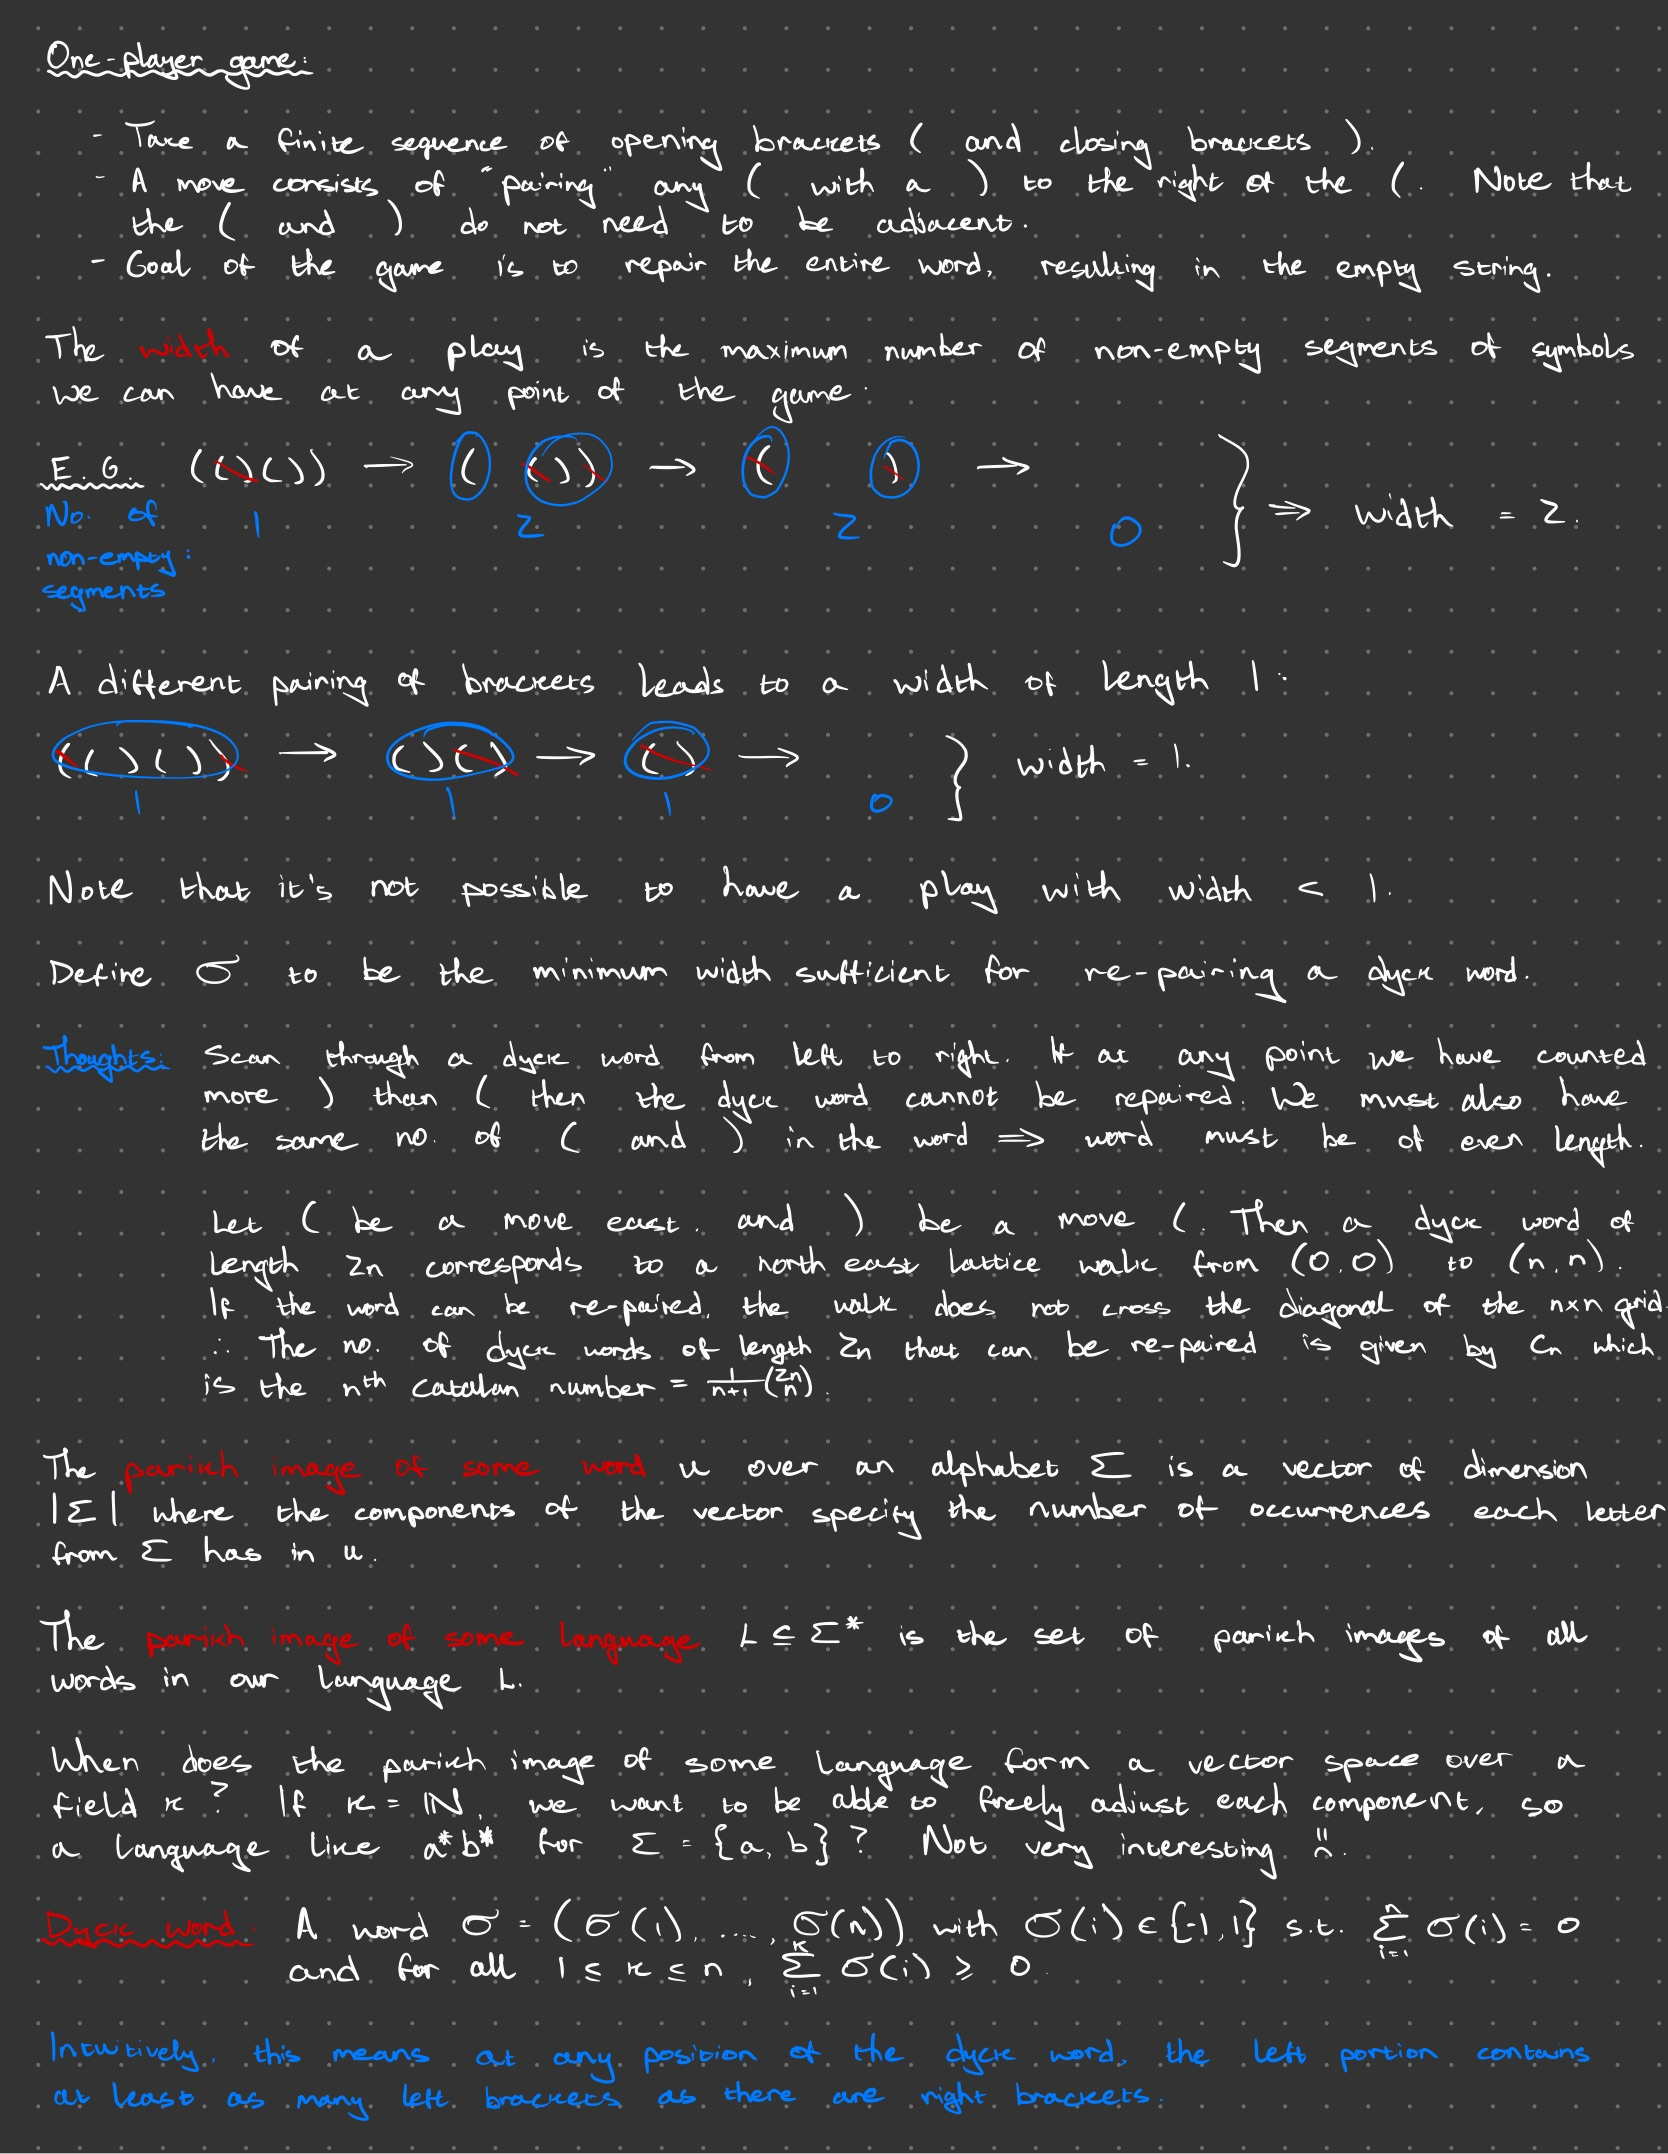
\includegraphics[scale=0.227]{./images/notesExample.jpg}
    \caption{An example page of the written notes taken}
\end{figure}